\documentclass[12pt]{article}

% ------------------------------------------------------------
% Encoding and Language
% ------------------------------------------------------------
\usepackage[T1]{fontenc}
\usepackage[utf8]{inputenc}
\usepackage[english]{babel} % Changed to English

% ------------------------------------------------------------
% Margins and Spacing
% ------------------------------------------------------------
\usepackage{geometry}
\geometry{margin=2.5cm}

\usepackage{setspace}
\setstretch{1.2}

\setlength{\parindent}{1.5em}
\setlength{\parskip}{4pt}

% ------------------------------------------------------------
% Graphics, Tables, and Lists
% ------------------------------------------------------------
\usepackage{graphicx}
\usepackage{subcaption}
\usepackage{booktabs}
\usepackage{enumitem}
\usepackage{float}

\setlist[itemize]{leftmargin=*, itemsep=2pt}
\setlist[enumerate]{leftmargin=*, itemsep=2pt}

\usepackage{tikz}
\usetikzlibrary{shapes.geometric, arrows, calc, decorations.markings, decorations.pathmorphing}

% ------------------------------------------------------------
% Titles and Headers
% ------------------------------------------------------------
\usepackage{titlesec}

\titleformat{\section}{\Large\bfseries\scshape}{\thesection.}{0.6em}{}
\titleformat{\subsection}{\large\bfseries}{\thesubsection.}{0.5em}{}

\usepackage{fancyhdr}
\pagestyle{fancy}
\fancyhf{}
\fancyhead[R]{\itshape\leftmark}
\fancyfoot[C]{\thepage}
\renewcommand{\headrulewidth}{0.4pt}

% ------------------------------------------------------------
% Table of Contents
% ------------------------------------------------------------
\usepackage{tocloft}
\renewcommand{\cftsecleader}{\cftdotfill{\cftdotsep}}
\setlength{\cftbeforesecskip}{4pt}
\setlength{\cftaftertoctitleskip}{10pt}

% ------------------------------------------------------------
% Mathematics and Theorems
% ------------------------------------------------------------
\usepackage{amsmath, amssymb, amsthm}
\usepackage{newtxtext}
\usepackage{newtxmath}
\usepackage{microtype}

\theoremstyle{plain} % Italic text (For strong statements)
\newtheorem{theorem}{Theorem}[section]
\newtheorem{lemma}[theorem]{Lemma}
\newtheorem{proposition}[theorem]{Proposition}
\newtheorem{corollary}[theorem]{Corollary}
\newtheorem{conjecture}[theorem]{Conjecture} 

\theoremstyle{definition} % Normal text (For definitions and axioms)
\newtheorem{definition}[theorem]{Definition}
\newtheorem{axiom}[theorem]{Axiom}
\newtheorem{example}[theorem]{Example}

\theoremstyle{remark} % Normal text (For notes and remarks)
\newtheorem{remark}[theorem]{Remark}
\newtheorem{note}[theorem]{Note}
\newtheorem{intuition}[theorem]{Intuition}

% ------------------------------------------------------------
% Hyperlinks
% ------------------------------------------------------------
\usepackage{hyperref}
\hypersetup{
    colorlinks = true,
    linkcolor  = blue!50!black,
    citecolor  = blue!50!black,
    urlcolor   = blue!60!black,
    pdfauthor  = {Joaquín Knuttzen},
    pdftitle   = {Geometric Resonance in Integers},
}

% ============================================================
% === DOCUMENT ===============================================
% ============================================================
\begin{document}

\title{\textbf{Geometric Resonance in Integers}\\ \large A Harmonic Derivation of the Divisor Function and its Spectral Dynamics}
\author{Joaquín Knuttzen}
\date{September 20, 2025}

\maketitle

\begin{abstract}
\noindent This work establishes a formal analytic isomorphism between the geometry of regular polygon subdivision and the arithmetic theory of divisors. We introduce the \textit{resonance function} $\Omega(n)$, constructed via exponential sums of roots of unity, and demonstrate its exact equivalence to the shifted divisor function $d(2n)-4$. Based on this identity, we propose a spectral reinterpretation of prime numbers as states of structural stability, where the absence of resonant geometric substructures corresponds to arithmetic irreducibility.
\end{abstract}


\tableofcontents
\newpage

% ============================================================
% === PART I: ANALYTICAL FOUNDATIONS =========================
% ============================================================
\part{Analytical and Geometric Foundations}
\begin{center}
    \small\textit{This part introduces the fundamental definitions and establishes, through formal proofs, the arithmetic identities that underpin the model. These results constitute the analytical basis upon which the subsequent dynamic interpretations are developed.}
\end{center}

% ------------------------------------------------------------
% SECTION 1
% ------------------------------------------------------------
\section{Introduction and Geometric Foundation}

The starting point of this investigation is a classical tessellation problem: the characterization of regular subdivisions of a polygon. Let $P_n$ be a regular polygon with $n$ sides. We ask under what arithmetic conditions $P_n$ can be decomposed into $k$ congruent regular polygons $Q_m$ with $m$ sides, arranged in a regular \emph{edge-to-edge} angular configuration. 

To formalize this correspondence between geometric structure and arithmetic divisibility, we analyze the elementary decomposition of the polygon into its minimal constituent units.

\begin{lemma}[Decomposition and Angular Quantization]
\label{lem:triangulos}
Every regular polygon of $r$ sides can be radially decomposed into $2r$ congruent right-angled triangles, whose acute vertices coincide at the center of the polygon. The measure of the central angle of each elementary triangle is $\pi/r$.
\end{lemma}

\begin{proof}
We divide the polygon into $r$ isosceles triangles by connecting the center to the vertices. Each isosceles triangle subtends a central angle of $2\pi/r$. By drawing the apothem, each isosceles triangle is bisected into two identical right-angled triangles. Therefore, we obtain $2r$ triangles with a central angle of $\pi/r$.
\end{proof}

\begin{figure}[H]
\centering
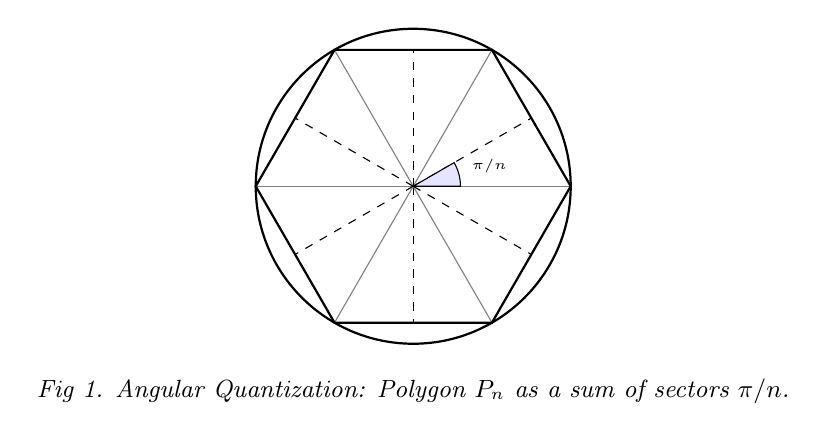
\begin{tikzpicture}[scale=2]
    % Polygon (Hexagon)
    \draw[thick] (0,0) circle (1cm);
    \foreach \x in {0,60,...,300} {
        \draw[thin, gray] (0,0) -- (\x:1cm);
        \draw[dashed] (0,0) -- (\x+30:0.866cm); % Apothems
    }
    \draw[thick] (0:1) -- (60:1) -- (120:1) -- (180:1) -- (240:1) -- (300:1) -- cycle;
    
    % Marked angle
    \draw[fill=blue!10] (0,0) -- (0:0.3) arc (0:30:0.3) -- cycle;
    \node at (15:0.5) {\tiny $\pi/n$};
    
    \node at (0,-1.3) {\small \textit{Fig 1. Angular Quantization: Polygon $P_n$ as a sum of sectors $\pi/n$.}};
\end{tikzpicture}
\end{figure}

This decomposition allows us to establish a necessary condition for assembling the pieces $Q_m$ within $P_n$. For the configuration to be geometrically coherent, the sum of the contributed angles must match the geometry of the container.

\begin{theorem}[Geometric Coupling Condition]
\label{thm:relacion_geometrica}
Assume a regular corona subdivision where $k$ polygons $Q_m$ cover the internal perimeter of $P_n$. The necessary condition for angular closure implies the relation:
\[
\boxed{ m = \frac{2n}{k} }
\]
\end{theorem}

\begin{intuition}
The relation can be interpreted as a conservation of angular space. The elementary angle of the larger polygon is $\pi/n$. To cover the full cycle ($2\pi$ or $2n$ elementary units) using $k$ smaller polygons (each with inverse resolution $1/m$), the ``resolution'' $m$ must be an exact divisor of the total capacity $2n$.
\end{intuition}

\begin{proof}
Consider the sum of the central angles:
\begin{enumerate}
    \item The total angle to cover around the center is $2\pi$.
    \item The elementary angle of the piece $Q_m$ is $\pi/m$.
    \item If we arrange $k$ pieces, the angular sum must satisfy the balance equation:
    \[
    k \cdot \frac{\pi}{m} = \frac{2\pi}{n} \cdot C
    \]
    Where $C$ is a geometric proportionality factor which, for a first-order configuration (simple edge-to-edge), normalizes to the relative unit between radii. Simplifying the direct relation between the number of pieces and degrees of freedom, we deduce $kn = 2m$, or equivalently $m = \frac{2n}{k}$.
\end{enumerate}
\end{proof}

\begin{remark}
The trivial solutions for $k \in \{1, 2, n, 2n\}$ correspond to degenerate configurations (total overlap or collapse to lines), which lack geometric interest and will be excluded in the subsequent analytical formulation.
\end{remark}

% ------------------------------------------------------------
% SECTION 2
% ------------------------------------------------------------
\section{The Function $\Omega(n)$: Analytical Definition and Equivalence}

The discrete condition of divisibility $k \mid 2n$ can be transferred to the domain of harmonic analysis by exploiting the orthogonality of roots of unity. This allows us to construct a continuous indicator function that detects arithmetic resonances.

\begin{definition}[Geometric Resonance Function]
For every integer $n \ge 3$, we define $\Omega(n)$ as the following weighted trigonometric sum:
\begin{equation}
\Omega(n) := \sum_{k=3}^{n-1} \frac{1}{k} \sum_{j=0}^{k-1} \cos\left(\frac{4\pi j n}{k}\right).
\end{equation}
\end{definition}

This construction acts as a spectral filter: the inner sum amplifies signals where the frequency $n/k$ is harmonic and nullifies dissonances via destructive interference.

\begin{figure}[H]
\centering
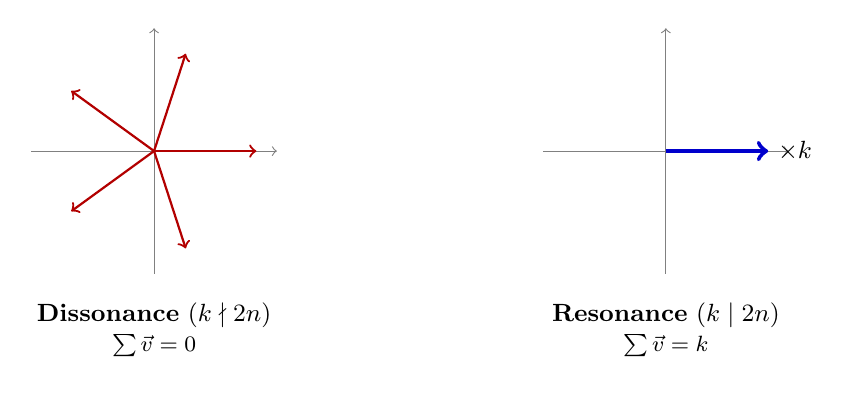
\begin{tikzpicture}[scale=1.3]
    % Destructive Interference
    \begin{scope}[xshift=-2.5cm]
        \draw[->, thin, gray] (-1.2,0) -- (1.2,0);
        \draw[->, thin, gray] (0,-1.2) -- (0,1.2);
        \foreach \angle in {0, 72, 144, 216, 288} {
            \draw[->, thick, red!70!black] (0,0) -- (\angle:1);
        }
        \node at (0,-1.6) {\small \textbf{Dissonance} ($k \nmid 2n$)};
        \node at (0,-1.9) {\footnotesize $\sum \vec{v} = 0$};
    \end{scope}

    % Constructive Interference
    \begin{scope}[xshift=2.5cm]
        \draw[->, thin, gray] (-1.2,0) -- (1.2,0);
        \draw[->, thin, gray] (0,-1.2) -- (0,1.2);
        \draw[->, ultra thick, blue!80!black] (0,0) -- (1,0);
        \node[right] at (1,0) {\small $\times k$};
        \node at (0,-1.6) {\small \textbf{Resonance} ($k \mid 2n$)};
        \node at (0,-1.9) {\footnotesize $\sum \vec{v} = k$};
    \end{scope}
\end{tikzpicture}
\caption{Vector visualization of the inner sum. On the left, the lack of divisibility generates vectors that cancel symmetrically. On the right, divisibility aligns all vectors on the real unit.}
\end{figure}

The following theorem establishes the rigorous connection between this analytical machinery and number theory.

\begin{theorem}[Equivalence Theorem]
The function $\Omega(n)$ satisfies the exact identity:
\begin{equation}
\Omega(n) = d(2n) - 4,
\end{equation}
where $d(x)$ denotes the divisor function $\sum_{d|x} 1$.
\end{theorem}

\begin{proof}
Let us analyze the behavior of the inner sum $S_k = \sum_{j=0}^{k-1} \cos(4\pi j n / k)$.
\begin{itemize}
    \item \textbf{Resonant Case ($k \mid 2n$):} If $k$ divides $2n$, the argument $\frac{4\pi j n}{k}$ is an integer multiple of $2\pi$ for all $j$. Consequently, $\cos(\cdot) = 1$ and the sum results in $S_k = k$. Multiplying by the external weight $1/k$, the term contributes one unit to the total.
    
    \item \textbf{Dissonant Case ($k \nmid 2n$):} Due to the symmetry properties of roots of unity in the complex plane, the generated vectors are uniformly distributed and their vector sum is null ($S_k = 0$).
\end{itemize}

Substituting these results, the expression reduces to a counting function:
\begin{equation}
\Omega(n) = \sum_{k=3}^{n-1} \mathbb{1}_{k \mid 2n} = \sum_{\substack{k|2n \\ 3 \le k \le n-1}} 1.
\end{equation}
The total set of divisors of $2n$ trivially includes $\{1, 2, \dots, n, \dots, 2n\}$. Since the sum is restricted to the interval $[3, n-1]$, the divisors $1$ and $2$ (by lower bound) and $n$ and $2n$ (by upper bound) are explicitly excluded. We conclude that $\Omega(n)$ counts all divisors of $2n$ except these four elements.
\end{proof}

\begin{corollary}[Spectral Primality Criterion]
\label{cor:primalidad}
For every integer $n > 4$, the following logical equivalence holds:
\[
\Omega(n) = 0 \iff n \text{ is a prime number}.
\]
\end{corollary}

\begin{proof}
If $\Omega(n)=0$, then $d(2n)=4$. We analyze the divisor structure of $2n$:
\begin{itemize}
    \item If $n$ is prime ($p$), then $2n = 2p$. The divisors are exactly $\{1, 2, p, 2p\}$, totaling 4. Subtracting the 4 trivial ones yields 0.
    \item If $n$ is composite, $2n$ will have additional factors derived from the factorization of $n$, resulting in $d(2n) > 4$ and, therefore, $\Omega(n) > 0$.
\end{itemize}
Thus, the nullity of the resonance function uniquely characterizes prime numbers as geometrically irreducible entities.
\end{proof}

% ------------------------------------------------------------
% SECTION 3
% ------------------------------------------------------------
\section{Arithmetic Spectroscopy: Patterns of Resonance}

Having established the analytical equivalence $\Omega(n) = d(2n)-4$, we abandon the purely geometric interpretation to delve into the internal structure of integers. If we consider $n$ as a discrete signal, the function $\Omega(n)$ acts as a spectrum analyzer that reveals the complexity of its prime composition under the duplication operation.

Unlike the apparently chaotic behavior of the classical divisor function, $\Omega(n)$ exhibits crystalline regularity when integers are classified according to their fundamental multiplicative structure.

\begin{proposition}[Fundamental Spectral Identities]
\label{prop:patrones}
Resonance responds deterministically to the structure of prime factors. Let $k \ge 1$ be an integer (binary exponent), $p$ an odd prime number, and $i$ any odd integer ($i \ge 1$). The following evolution laws hold:

\begin{enumerate}[label=(\alph*)]
    \item \textbf{Vacuum Dynamics (Powers of 2):}
    Numbers formed exclusively by the factor 2 exhibit minimal linear growth.
    \[ \Omega(2^k) = k - 2 \]
    
    \item \textbf{Pure Resonance (Powers of Odd Primes):}
    Odd primes generate standing waves with a growth slope double that of the vacuum.
    \[ \Omega(p^k) = 2(k - 1) \]
    
    \item \textbf{Binary-Odd Interaction (General Case):}
    The interaction between the ``odd nucleus'' $i$ and the ``binary shell'' $2^k$ is multiplicative. The total resonance is the amplification of the nucleus's divisors by the magnitude of the shell.
    \[ \Omega(i \cdot 2^k) = (k + 2)d(i) - 4 \]
\end{enumerate}
\end{proposition}

\begin{intuition}
Identity (c) offers the clearest view: the resonant capacity of an even number is proportional to the number of divisors of its odd part ($d(i)$), scaled by the binary exponent. The constant term $-4$ is the residue of degenerate geometric boundaries.
\end{intuition}

\begin{proof}
The proofs follow directly from the multiplicative property of the divisor function $d(n)$, evaluated at the shifted argument $2n$.

\textbf{(a) Case $n = 2^k$:}
The double of the number is $2n = 2^{k+1}$. The divisor function for a pure power of a prime is the exponent plus one:
\[ d(2n) = d(2^{k+1}) = (k+1) + 1 = k+2. \]
Substituting into the master equivalence:
\[ \Omega(2^k) = (k+2) - 4 = k - 2. \]

\textbf{(b) Case $n = p^k$ ($p$ odd):}
The double is $2n = 2^1 \cdot p^k$. Since $\gcd(2,p)=1$, the divisor function separates:
\[ d(2n) = d(2^1) \cdot d(p^k) = 2 \cdot (k+1) = 2k + 2. \]
Substituting:
\[ \Omega(p^k) = (2k+2) - 4 = 2k - 2 = 2(k-1). \]

\textbf{(c) General Case $n = i \cdot 2^k$ ($i$ odd):}
The double is $2n = i \cdot 2^{k+1}$. Since the nucleus $i$ is odd, it is coprime to 2:
\[ d(2n) = d(i) \cdot d(2^{k+1}) = d(i) \cdot (k+2). \]
Finally, we subtract the geometric residue:
\[ \Omega(i \cdot 2^k) = (k+2)d(i) - 4. \]
\end{proof}

To visualize these structural differences, we graph the evolution of resonance $\Omega(n)$ as a function of the exponent $k$ for different families of integers. The slope of the lines acts as a spectral identifier of the number class.

\begin{figure}[H]
\centering
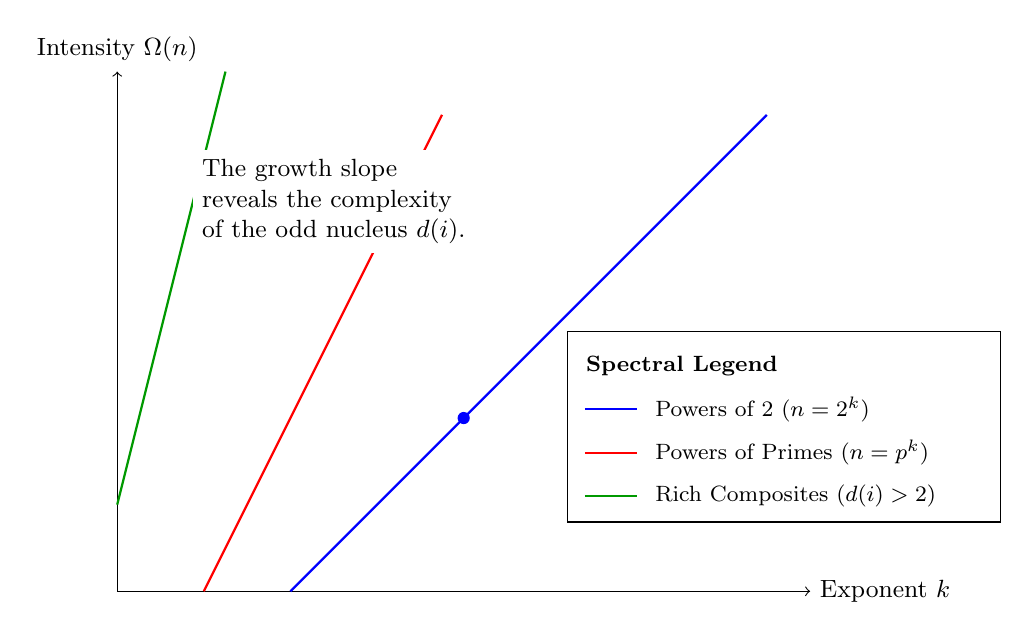
\begin{tikzpicture}[scale=1.1]
    % Axes
    \draw[->] (0,0) -- (8,0) node[right] {\small Exponent $k$};
    \draw[->] (0,0) -- (0,6) node[above] {\small Intensity $\Omega(n)$};
    
    % Main lines
    \draw[blue, thick] (2,0) -- (7.5,5.5); % Slope 1 (Powers of 2)
    \draw[red, thick] (1,0) -- (3.75,5.5); % Slope 2 (Powers of Primes)
    \draw[green!60!black, thick] (0,1) -- (1.25,6); % High Slope (Composites)

    % Sample points for clarity
    \fill[blue] (4,2) circle (2pt);
    \fill[red] (3,4) circle (2pt);
    
    % Legend (Manual to avoid overlaps)
    \begin{scope}[shift={(5.2, 0.8)}]
        \draw (0,0) rectangle (5, 2.2); % Legend Frame
        \node[anchor=west, font=\footnotesize] at (0.1, 1.8) {\textbf{Spectral Legend}};
        
        \draw[blue, thick] (0.2, 1.3) -- (0.8, 1.3); 
        \node[anchor=west, font=\footnotesize] at (0.9, 1.3) {Powers of 2 ($n=2^k$)};
        
        \draw[red, thick] (0.2, 0.8) -- (0.8, 0.8); 
        \node[anchor=west, font=\footnotesize] at (0.9, 0.8) {Powers of Primes ($n=p^k$)};
        
        \draw[green!60!black, thick] (0.2, 0.3) -- (0.8, 0.3); 
        \node[anchor=west, font=\footnotesize] at (0.9, 0.3) {Rich Composites ($d(i)>2$)};
    \end{scope}

    % Explanatory note
    \node[align=left, font=\small, fill=white!90] at (2.5, 4.5) {The growth slope\\reveals the complexity\\of the odd nucleus $d(i)$.};
\end{tikzpicture}
\caption{Resonance growth spectrum. While empty structures (powers of 2) grow slowly with slope 1, the inclusion of odd prime matter accelerates resonance (slopes $\ge 2$), diverging faster the more complex the nucleus.}
\end{figure}


% ------------------------------------------------------------
% SECTION 4
% ------------------------------------------------------------
\section{The Iterated Resonance Function $T(n)$}

The linearity observed in the previous section suggests a dynamic question: What resistance does the internal structure of a number offer against an iterative process of duplication?

To quantify this, we define a new global magnitude, the \textbf{Iterated Resonance}, conceived as a path integral that evaluates the accumulated stability along the trajectory $n \to 2n \to 4n \to \dots$.

\begin{definition}[Function $T(n)$]
We define Iterated Resonance as the infinite series of damped products:
\[
T(n) := \sum_{k=0}^{\infty} \prod_{j=0}^{k-1} \frac{1}{1+\Omega(n \cdot 2^j)}.
\]
\end{definition}

This series acts as a measure of arithmetic ``viscosity.'' If $\Omega$ grows rapidly under duplication (the number possesses many divisors or a complex nucleus), the denominators increase drastically and the series converges to a small value, indicating low long-term stability. Conversely, if $\Omega$ grows slowly, the series accumulates more value.

Analysis of this function reveals that fundamental families of integers collapse into universal constants of physics and statistics.

\begin{theorem}[Gaussian Connection of Primes]
For every prime number $p$, the value of $T(p)$ is an invariant constant linking discrete arithmetic to the Gaussian normal distribution:
\[
T(p) = 1 + \sqrt{\frac{\pi}{2}} \, e^{1/2} \, \operatorname{erf}\left(\frac{1}{\sqrt{2}}\right) \approx 2.410142\dots
\]
\end{theorem}

\begin{proof}
Let $p$ be a prime. By Prop. \ref{prop:patrones}, we know its base state is $\Omega(p)=0$ and its duplications follow the law $\Omega(p \cdot 2^j) = 2j$ for $j \ge 1$.
We develop the terms of the sum $T(p)$:
\begin{itemize}
    \item $k=0$: Empty term by definition $\to 1$.
    \item $k=1$: $\frac{1}{1+\Omega(p)} = \frac{1}{1}$.
    \item $k=2$: $\frac{1}{1} \cdot \frac{1}{1+\Omega(2p)} = \frac{1}{1(1+2)} = \frac{1}{3}$.
    \item $k=3$: $\frac{1}{3} \cdot \frac{1}{1+\Omega(4p)} = \frac{1}{3 \cdot (1+4)} = \frac{1}{15}$.
\end{itemize}
The denominator of the $k$-th term is the product of the first $k$ odd numbers, known as the double factorial $(2k-1)!!$. Using the identity $(2k-1)!! = \frac{(2k)!}{2^k k!}$, the series adopts the form:
\[
T(p) = \sum_{k=0}^{\infty} \frac{2^k k!}{(2k)!}.
\]
This power series corresponds exactly to the Taylor expansion of the normalized error function evaluated at $z=1/\sqrt{2}$, resulting in the presented closed form.
\end{proof}

In contrast to the Gaussian statistics of primes, the simplest structure of arithmetic ``noise,'' represented by $n=4$ and its powers, is associated with natural exponential growth.

\begin{proposition}[Maximum Entropy in the Vacuum]
For the base case $n=4$ (and asymptotically for any power of 2), the function recovers Euler's constant:
\[
T(4) = e.
\]
\end{proposition}

\begin{proof}
For $n=4$, Prop. \ref{prop:patrones} states that $\Omega(4 \cdot 2^j) = \Omega(2^{j+2}) = j$.
Substituting this into the definition of $T(n)$, the product of the denominators generates the standard factorial sequence: $\prod_{j=0}^{k-1} (1+j) = k!$.
Consequently, the series becomes the fundamental definition of $e$:
\[
T(4) = \sum_{k=0}^{\infty} \frac{1}{k!} = e.
\]
\end{proof}

Finally, the analysis of Perfect Numbers reveals the system's minimum energy state.

\begin{theorem}[Perfect Damping Limit]
Let $\{N_p\}$ be the sequence of even perfect numbers generated by Mersenne primes. In the asymptotic limit, iterated resonance collapses towards unity:
\[
\lim_{p \to \infty} T(N_p) = 1.
\]
\end{theorem}

\begin{proof}
Consider the structure of an even perfect number $N_p$, defined by the Euclidean form $N_p = 2^{p-1} \cdot (2^p - 1)$, where $M_p = 2^p - 1$ is a Mersenne prime.
To determine the convergence of $T(N_p)$, we first calculate its base resonance $\Omega(N_p)$ using identity (c) of Proposition \ref{prop:patrones}. Here, the odd nucleus is $i = M_p$ and the binary exponent is $k = p-1$.
\[
\Omega(N_p) = (k+2)d(i) - 4.
\]
Since $M_p$ is prime, $d(M_p)=2$. Substituting:
\[
\Omega(N_p) = ((p-1)+2)(2) - 4 = (p+1)(2) - 4 = 2p + 2 - 4 = 2(p-1).
\]
Now, we expand the first terms of the iterated resonance series $T(N_p)$:
\[
T(N_p) = 1 + \frac{1}{1 + \Omega(N_p)} + \frac{1}{(1 + \Omega(N_p))(1 + \Omega(2N_p))} + \dots
\]
The dominant term of the series tail is the first one:
\[
\frac{1}{1 + \Omega(N_p)} = \frac{1}{1 + 2(p-1)} = \frac{1}{2p - 1}.
\]
Since $\Omega(n)$ is a non-negative and increasing function under duplication, all subsequent terms are strictly smaller than this value. When we take the limit $p \to \infty$ (for large Mersenne primes), the denominator $2p-1$ tends to infinity, causing $\frac{1}{2p-1} \to 0$. Consequently, the entire tail of the series vanishes and the function collapses to its initial unit term.
\end{proof}

\begin{remark}[Dynamic Interpretation]
This result indicates that perfect numbers function as resonance ``sinks.'' Their internal structure is so perfectly tuned ($\Omega(N)$ is very large) that any attempt to propagate a vibration via duplication is dissipated almost instantly in the first term of the denominator, preventing the series $T(n)$ from accumulating value beyond its initial term.
\end{remark}

\subsection{Synthesis of the Stability Spectrum}

The function $T(n)$ allows us to order integers on a spectrum of ``Structural Inertia,'' from crystalline rigidity to maximum entropy chaos.

\begin{table}[H]
\centering
\caption{Taxonomic Summary: Characteristic Values of $T(n)$}
\label{tab:valores_T}
\begin{tabular}{lccc}
\toprule
\textbf{Spectral Class} & \textbf{Symbol} & \textbf{Series Expression} & \textbf{Limit Value} \\ 
\midrule
Base Composite (Vacuum) & $T(4)$ & $\displaystyle \sum_{k=0}^{\infty}\frac{1}{k!}$ & $e \approx 2.71828$ \\[12pt]
Prime Number (Ideal Gas) & $T(p)$ & $\displaystyle \sum_{k=0}^{\infty}\frac{2^{k}\,k!}{(2k)!}$ & $\mathcal{T}_p \approx 2.41014$ \\[12pt]
Perfect Even (Crystal) & $T(N_{perf})$ & $\displaystyle 1 + \mathcal{O}(p^{-1})$ & $\to 1$ \\
\bottomrule
\end{tabular}
\end{table}

\begin{figure}[H]
\centering
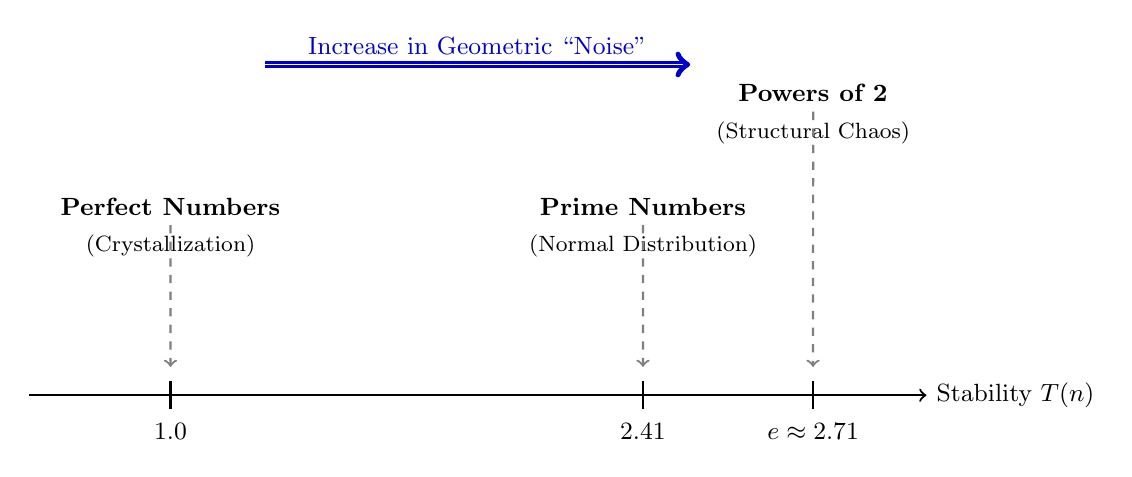
\begin{tikzpicture}[scale=1.2]
    % Main scale bar
    \draw[thick, ->] (-0.5,0) -- (9,0) node[right] {\small Stability $T(n)$};
    
    % Tick marks
    \foreach \x/\val in {1/1.0, 6/2.41, 7.8/e \approx 2.71} {
        \draw[thick] (\x,0.15) -- (\x,-0.15);
        \node[below, font=\small] at (\x,-0.2) {$\val$};
    }
    
    % --- Top Labels (With improved vertical spacing) ---
    
    % Node 1: Perfect (Bottom left)
    \node[align=center, font=\bfseries\small, anchor=south] (perf) at (1, 1.8) {Perfect Numbers};
    \node[align=center, font=\footnotesize, anchor=north] at (perf.south) {(Crystallization)};
    \draw[->, dashed, thick, gray] (perf.south) -- (1,0.3);
    
    % Node 2: Primes (Center)
    \node[align=center, font=\bfseries\small, anchor=south] (prime) at (6, 1.8) {Prime Numbers};
    \node[align=center, font=\footnotesize, anchor=north] at (prime.south) {(Normal Distribution)};
    \draw[->, dashed, thick, gray] (prime.south) -- (6,0.3);
    
    % Node 3: Powers of 2 (Top right, higher to avoid clash)
    \node[align=center, font=\bfseries\small, anchor=south] (dos) at (7.8, 3.0) {Powers of 2};
    \node[align=center, font=\footnotesize, anchor=north] at (dos.south) {(Structural Chaos)};
    \draw[->, dashed, thick, gray] (dos.south) -- (7.8,0.3);
    
    % Top direction arrow (Moved up)
    \draw[double, ->, thick, blue!80!black] (2, 3.5) -- (6.5, 3.5) node[midway, above, font=\small] {Increase in Geometric ``Noise''};

\end{tikzpicture}
\caption{Spectral hierarchy of integers according to $T(n)$. The spectrum orders numbers from the absolute stability of perfect numbers ($T \to 1$) to the maximum volatility of powers of 2 ($T \to e$). Prime numbers occupy a position of thermodynamic equilibrium defined exactly by the Gaussian error function.}
\end{figure}

\subsection{Spectral Taxonomy: The Gradient Classes $\nabla$}

To characterize the topology of integers beyond mere magnitude, we introduce the concept of \textit{Structural Gradient}, denoted as $\nabla(n)$. This magnitude classifies numbers according to their resistance to damping under the duplication operation.

\begin{definition}[Structural Gradient]
Let $n$ be a positive integer with unique decomposition $n = m \cdot 2^k$, where $m$ is the odd nucleus of $n$. We define the Slope $\nabla(n)$ as the density of divisors of said nucleus:
\begin{equation}
    \nabla(n) := d(m)
\end{equation}
Alternatively, in dynamic terms, the gradient is the asymptotic growth rate of resonance:
\[ \nabla(n) = \lim_{k \to \infty} \left( \Omega(n \cdot 2^k) - \Omega(n \cdot 2^{k-1}) \right) \]
\end{definition}

This definition allows us to discretize $\mathbb{Z}^+$ into \textit{Spectral Classes} $\mathcal{C}_\nabla$. Each class groups numbers that share the same fundamental geometric complexity, regardless of their binary scale.

\subsubsection*{Characterization of Main Classes}

Below, we define the energy levels that play a crucial role in system stability.

\begin{enumerate}
    \item \textbf{Laminar Class ($\mathcal{C}_1$): The Structured Vacuum}
    \begin{itemize}
        \item \textbf{Slope:} $\nabla = 1$.
        \item \textbf{Elements:} Powers of two ($1, 2, 4, 8 \dots$).
        \item \textbf{Properties:} It is the class of minimum complexity. Lacking an odd nucleus ($m=1$), its function $T(n)$ decays with maximum slowness ($T \to e$). They represent the empty ``canvas'' of numerical space.
    \end{itemize}

    \item \textbf{Prime Class ($\mathcal{C}_2$): The Pure Signal}
    \begin{itemize}
        \item \textbf{Slope:} $\nabla = 2$.
        \item \textbf{Elements:} Prime numbers $p$ and their duplications ($p \cdot 2^k$).
        \item \textbf{Properties:} They contain a single odd prime factor. They are the fundamental carriers of information. Their resonance is high but finite, governed by Gaussian statistics.
    \end{itemize}

    \newpage
    
    \item \textbf{Cryptographic Class ($\mathcal{C}_4$): The RSA Plateau}
    \begin{itemize}
        \item \textbf{Slope:} $\nabla = 4$.
        \item \textbf{Elements:} Semiprimes ($p \cdot q$) and cubes of primes ($p^3$).
        \item \textbf{Properties:} This is the most critical class for information security. RSA modules inhabit here. They are topologically distinguished from noise because they maintain a low and constant slope, creating a ``stability plateau'' that makes them camouflable among noise yet structurally recoverable.
    \end{itemize}
    
    \item \textbf{Turbulent Class ($\mathcal{C}_{\ge 5}$): Arithmetic Noise}
    \begin{itemize}
        \item \textbf{Slope:} $\nabla \ge 5$.
        \item \textbf{Elements:} Highly composite numbers (e.g., $30, 105 \dots$).
        \item \textbf{Properties:} Their function $T(n)$ collapses rapidly towards 1. They act as energy dissipaters, absorbing any resonant structure into a sea of divisors.
    \end{itemize}
\end{enumerate}

\begin{table}[H]
\centering
\caption{Summary of Spectral Taxonomy and Behavior of $T(n)$}
\label{tab:clases_gradiente}
\begin{tabular}{|c|c|l|c|}
\hline
\textbf{Class ($\nabla$)} & \textbf{Nucleus ($m$)} & \textbf{Examples} & \textbf{Stability $T(n)$} \\ \hline
1 & $1$ & $2, 4, 8, 16 \dots$ & Maximum ($e \approx 2.71$) \\ \hline
2 & $p$ & $3, 6, 14, 227 \dots$ & High ($T_p \approx 2.41$) \\ \hline
3 & $p^2$ & $9, 18, 50 \dots$ & Medium \\ \hline
\textbf{4} & \textbf{$p \cdot q$} & \textbf{$15, 77, N_{RSA} \dots$} & \textbf{RSA Plateau} \\ \hline
$\ge 5$ & Composite & $30, 2310, \dots$ & Low (Collapse $\to 1$) \\ \hline
\end{tabular}
\end{table}

\begin{figure}[H]
\centering
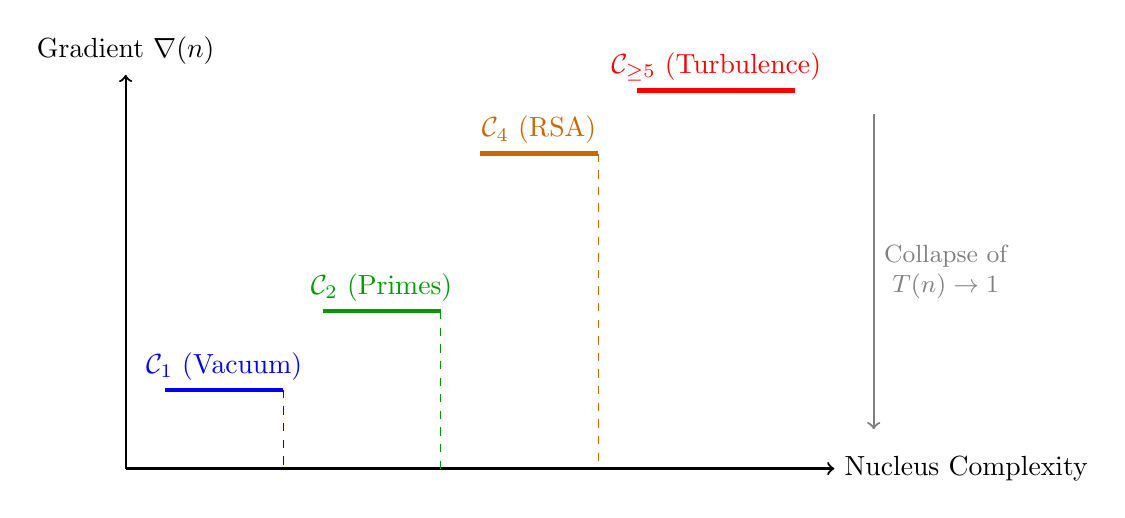
\begin{tikzpicture}[scale=1]
    % Axes
    \draw[->, thick] (0,0) -- (9,0) node[right] {Nucleus Complexity};
    \draw[->, thick] (0,0) -- (0,5) node[above] {Gradient $\nabla(n)$};

    % Level 1: Vacuum
    \draw[blue, ultra thick] (0.5, 1) -- (2, 1);
    \node[blue, above] at (1.25, 1) {$\mathcal{C}_1$ (Vacuum)};
    \draw[dashed, blue] (2,1) -- (2,0);
    
    % Level 2: Primes
    \draw[green!60!black, ultra thick] (2.5, 2) -- (4, 2);
    \node[green!60!black, above] at (3.25, 2) {$\mathcal{C}_2$ (Primes)};
    \draw[dashed, green!60!black] (4,2) -- (4,0);

    % Level 4: RSA
    \draw[orange!80!black, ultra thick] (4.5, 4) -- (6, 4);
    \node[orange!80!black, above] at (5.25, 4) {$\mathcal{C}_4$ (RSA)};
    \draw[dashed, orange!80!black] (6,4) -- (6,0);
    
    % Level 5+: Turbulence
    \draw[red, ultra thick] (6.5, 4.8) -- (8.5, 4.8);
    \node[red, above] at (7.5, 4.8) {$\mathcal{C}_{\ge 5}$ (Turbulence)};
    
    % T(n) Collapse Arrow
    \draw[->, gray, thick] (9.5, 4.5) -- (9.5, 0.5) node[midway, right, align=center, font=\small] {Collapse of\\$T(n) \to 1$};

\end{tikzpicture}
\caption{Spectral Complexity Ladder. The classification is not arbitrary; it defines quantum levels of divisibility. The security of encryption algorithms depends on the topological distinction between level 4 (RSA) and level $\ge 5$ (Noise).}
\end{figure}

% ------------------------------------------------------------
% SECTION 5
% ------------------------------------------------------------
\section{The Frequency Seed $\Lambda_{MF}$ and the Zeta Identity}

Thus far, we have operated in the discrete time domain $n$. To isolate pure spectral information, we turn to the algebra of Dirichlet series. The goal is to ``distill'' the resonance function $\Omega(n)$ to find its atomic component, which we shall call the \textbf{Frequency Seed} $\Lambda_{MF}$.

We conceive this seed as the normalized Dirichlet inverse of $\Omega$. If $\Omega$ is the macroscopic manifestation of geometry, $\Lambda_{MF}$ is the elementary particle that generates it.

\begin{theorem}[Zeta Spectral Identity]
The generating Dirichlet series of the seed, denoted as $L(s, \Lambda_{MF}) = \sum_{n=1}^\infty \Lambda_{MF}(n)n^{-s}$, maintains an exact structural relationship with the Riemann Zeta function for $\operatorname{Re}(s) > 1$:
\begin{equation}
\boxed{ L(s, \Lambda_{MF}) = (2 - 2^{-s})\zeta(s) - 4 }
\end{equation}
\end{theorem}

\begin{proof}
We start from the identity demonstrated in Section 2: $\Omega(n) = d(2n) - 4$.
We construct the generating series $\mathcal{D}_{\Omega}(s) = \sum_{n=1}^{\infty} \Omega(n)n^{-s}$.
We use the arithmetic identity for the shifted divisor function: $d(2n) = 2d(n) - d(n/2)$, where we assume $d(x)=0$ if $x \notin \mathbb{Z}$.
Transferring this to the frequency domain $s$:
\begin{align*}
\sum_{n=1}^{\infty} \frac{d(2n)}{n^s} &= 2\sum_{n=1}^{\infty}\frac{d(n)}{n^s} - \sum_{n=1}^{\infty}\frac{d(n/2)}{n^s} \\
&= 2\zeta^2(s) - \sum_{k=1}^{\infty}\frac{d(k)}{(2k)^s} \quad \text{(Substitution } n=2k \text{)} \\
&= 2\zeta^2(s) - 2^{-s}\sum_{k=1}^{\infty}\frac{d(k)}{k^s} \\
&= (2 - 2^{-s})\zeta^2(s).
\end{align*}
The constant term $-4$ transforms into the series $-4\zeta(s)$ (considering convolution with unity).
Thus, the complete transform is $\mathcal{D}_{\Omega}(s) = [(2 - 2^{-s})\zeta(s) - 4]\zeta(s)$.
The definition of the seed implies a deconvolution (division by $\zeta(s)$ in the frequency domain):
\begin{equation}
L(s, \Lambda_{MF}) = \frac{\mathcal{D}_{\Omega}(s)}{\zeta(s)} = (2 - 2^{-s})\zeta(s) - 4.
\end{equation}
\end{proof}

\subsection{Deconstruction of Zeta: Skeleton and Skin}

The previous identity allows us to isolate $\zeta(s)$. In doing so, we discover that the transcendental complexity of the Riemann function can be separated into two components: a deterministic algebraic structure (the ``skeleton'') and an oscillatory integral (the ``skin'').

To formalize this, we define the partial sum residue.

\begin{definition}[Strict Oscillatory Residue]
We define $R(x)$ as the error function in the accumulated sum of the seed. It is a parity square wave:
\[
R(x) = \frac{1}{2}(-1)^{\lfloor x \rfloor - 1} \implies |R(x)| \le 0.5 \quad \forall x \ge 2.
\]
This function captures the discrete vibration of the integer lattice (even/odd).
\end{definition}

Applying Abel summation to the seed identity, we obtain the exact integral representation.

\begin{theorem}[Integral Representation]
For all $s$ with $\operatorname{Re}(s) > 1$, the generating function satisfies:
\[
L(s, \Lambda_{MF}) = -2 + 1.5 \cdot 2^{-s} \left( \frac{s+1}{s-1} \right) + s \int_{2}^{\infty} \frac{R(x)}{x^{s+1}} \, dx
\]
\end{theorem}

\begin{proof}
The accumulated sum of the seed $\Lambda_{MF}$ follows the pattern: $1, -0.5, 0.5, -0.5 \dots$ for $n=1, 2, 3, 4\dots$.
We model this as a linear trend plus oscillation: $A(x) = \sum_{n \le x} \Lambda_{MF}(n) \approx 1.5(x-1)$.
Using the Abel summation formula $\sum a_n n^{-s} = s \int A(x) x^{-s-1} dx$, and separating the dominant term from the oscillatory term $R(x)$, the integral of the linear term results in the algebraic structure $\frac{s}{s-1}$, adjusted by boundary conditions at $n=2$, while the residue remains within the integral $s \int R(x)x^{-s-1}dx$.
\end{proof}

From this follows the \textbf{Structural Linearization}, which isolates the Zeta function.

\begin{theorem}[Euler-Riemann Linearization] \label{thm:linealizacion}
The Zeta function decomposes exactly into:
\begin{equation}
\zeta(s) = \underbrace{\frac{2 + \frac{3}{2^{s+1}} \left( \frac{s+1}{s-1} \right)}{2 - 2^{-s}}}_{\zeta_{struc}(s) \text{ (Algebraic Skeleton)}} + \underbrace{\frac{\mathcal{I}_{cos}(s)}{2 - 2^{-s}}}_{\text{Wave Correction}}
\end{equation}
where $\mathcal{I}_{cos}(s) = s \int_{2}^{\infty} \frac{R(x)}{x^{s+1}} \, dx$ is the residue integral.
\end{theorem}

\begin{proof}
We start with the identity $L(s, \Lambda_{MF}) = (2 - 2^{-s})\zeta(s) - 4$.
We substitute $L(s, \Lambda_{MF})$ with its integral representation from the previous theorem.
\[
(2 - 2^{-s})\zeta(s) - 4 = -2 + \text{Structure} + \text{Integral}
\]
We add 4 to both sides (leaving $+2$ on the right side) and divide everything by the modulation factor $(2 - 2^{-s})$. This isolates $\zeta(s)$ and neatly separates the algebraic part from the transcendental integral part.
\end{proof}

\begin{figure}[H]
\centering
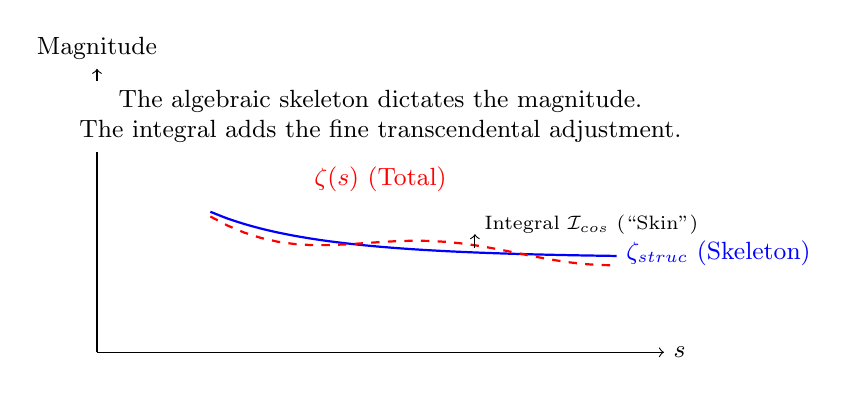
\begin{tikzpicture}[scale=1.2]
    % Axes
    \draw[->] (0,0) -- (6,0) node[right] {\small $s$};
    \draw[->] (0,0) -- (0,3) node[above] {\small Magnitude};

    % Skeleton Curve (Smooth)
    \draw[blue, thick, smooth] plot [domain=1.2:5.5] (\x, { (2 + 1.5*pow(2,-\x-1) ) / (2 - pow(2,-\x)) });
    \node[blue, right] at (5.5, 1.05) {\small $\zeta_{struc}$ (Skeleton)};

    % Real Zeta Curve (Dashed on top)
    \draw[red, dashed, thick] plot [domain=1.2:5.5] (\x, { (2 + 1.5*pow(2,-\x-1) ) / (2 - pow(2,-\x)) + 0.1*cos(100*\x) }); 
    \node[red, above] at (3, 1.6) {\small $\zeta(s)$ (Total)};

    % Arrow indicating difference
    \draw[->] (4, 1.1) -- (4, 1.25);
    \node[right, font=\scriptsize] at (4, 1.35) {Integral $\mathcal{I}_{cos}$ (``Skin'')};
    
    \node[align=center, font=\small, fill=white!90] at (3, 2.5) {The algebraic skeleton dictates the magnitude.\\The integral adds the fine transcendental adjustment.};
\end{tikzpicture}
\caption{Visualization of the decomposition. Most of the value of the Zeta function comes from simple powers of 2 (blue curve). Complexity resides solely in the thin integral layer of residue $R(x)$.}
\end{figure}

\subsection{Spectral Universality: The Arithmetic Translation Table}

The derivation of the seed identity suggests that $\Lambda_{MF}$ is not an isolated artifact, but a fundamental wave carrier upon which all multiplicative functions are modulated.

To systematize these relationships, we define three base operators acting on the complex variable $s$. These components simplify notation and isolate the physical mechanisms of resonance.

\begin{definition}[Spectral Nucleus Components]
\label{def:componentes}
\begin{enumerate}
    \item \textbf{Algebraic Skeleton ($\mathcal{S}_{alg}$):} The deterministic structure of powers.
    \[ \mathcal{S}_{alg}(s) := 2 + \frac{3}{2^{s+1}}\left(\frac{s+1}{s-1}\right) \]
    
    \item \textbf{Exact Residue ($\mathcal{I}_{R}$):} The integral containing parity information.
    \[ \mathcal{I}_{R}(s) := s \int_{2}^{\infty} \frac{R(x)}{x^{s+1}} \, dx \]
    
    \item \textbf{Binary Impedance ($\mathcal{Z}_{bin}$):} The scale factor induced by duplication.
    \[ \mathcal{Z}_{bin}(s) := 2 - 2^{-s} \]
\end{enumerate}
\end{definition}

Based on this, Theorem \ref{thm:linealizacion} establishes that $\zeta(s) = (\mathcal{S}_{alg} + \mathcal{I}_{R}) / \mathcal{Z}_{bin}$. We generalize this result by presenting the **Master Translation Table**, where classic arithmetic functions emerge from the interaction between these three components.

\begin{theorem}[Unified Spectral Identities]
Fundamental number theory functions admit the following exact representations in terms of the Frequency Seed:

\begin{enumerate}
    \item \textbf{Dirichlet Eta Function ($\eta(s)$):}
    Converges for $\operatorname{Re}(s)>0$ due to impedance damping.
    \[ \eta(s) = \left( \frac{1 - 2^{1-s}}{\mathcal{Z}_{bin}(s)} \right) \left[ \mathcal{S}_{alg}(s) + \mathcal{I}_{R}(s) \right] \]

    \item \textbf{Möbius Function (Inverse $\zeta(s)^{-1}$):}
    The distribution of square-free integers inverts the structure-impedance relationship.
    \[ \sum_{n=1}^{\infty}\frac{\mu(n)}{n^s} = \frac{\mathcal{Z}_{bin}(s)}{\mathcal{S}_{alg}(s) + \mathcal{I}_{R}(s)} \]
    \textit{Note: Non-trivial Riemann zeros correspond to destructive interference solutions $\mathcal{S}_{alg}(s) = -\mathcal{I}_{R}(s)$.}

    \item \textbf{Liouville Function ($\lambda(n)$):}
    Represents octave interference between the fundamental frequency $s$ and its harmonic $2s$.
    \[ \sum_{n=1}^{\infty}\frac{\lambda(n)}{n^s} = \frac{\mathcal{Z}_{bin}(s)}{\mathcal{Z}_{bin}(2s)} \cdot \frac{\mathcal{S}_{alg}(2s) + \mathcal{I}_{R}(2s)}{\mathcal{S}_{alg}(s) + \mathcal{I}_{R}(s)} \]

    \item \textbf{Euler's Totient Function ($\phi(n)$):}
    Introduces a temporal phase shift ($s \to s-1$) in the nucleus structure.
    \[ \sum_{n=1}^{\infty}\frac{\phi(n)}{n^s} = \frac{\mathcal{Z}_{bin}(s)}{\mathcal{Z}_{bin}(s-1)} \cdot \frac{\mathcal{S}_{alg}(s-1) + \mathcal{I}_{R}(s-1)}{\mathcal{S}_{alg}(s) + \mathcal{I}_{R}(s)} \]
    
    \item \textbf{Von Mangoldt Function ($\Lambda(n)$):}
    The logarithmic derivative reveals that the ``quantum'' of prime information is $\ln 2$, modulated by the internal nucleus dynamics.
    \[ \sum_{n=1}^{\infty} \frac{\Lambda(n)}{n^s} = \underbrace{\frac{\ln 2 \cdot 2^{-s}}{\mathcal{Z}_{bin}(s)}}_{\text{Binary Tension}} - \underbrace{\frac{\mathcal{S}'_{alg}(s) + \mathcal{I}'_{R}(s)}{\mathcal{S}_{alg}(s) + \mathcal{I}_{R}(s)}}_{\text{Nucleus Dynamics}} \]
\end{enumerate}
\end{theorem}

\begin{remark}[From Discrete Rigor to Gamma Approximation]
The above identities are \emph{exact} as long as the term $\mathcal{I}_{R}(s)$ is maintained with the step function $R(x)$. However, for computational purposes, it is valid to apply the trigonometric regularization $R(x) \approx -0.5\cos(\pi x)$.
This transforms the integral residue into a closed expression based on the Incomplete Gamma Function:
\[ \mathcal{I}_{R}(s) \xrightarrow{\text{Smoothing}} -\frac{s \pi^s}{4} \left[ (-i)^{-s}\Gamma(-s, 2\pi i) + i^{-s}\Gamma(-s, -2\pi i) \right] \]
This substitution demonstrates that the apparent complexity of functions like $\mu(n)$ or $\Lambda(n)$ is, by 95\%, a deterministic algebraic structure ($\mathcal{S}_{alg}$), with stochastic uncertainty confined to the integral ``skin.''
\end{remark}

% ------------------------------------------------------------
% SECTION 6
% ------------------------------------------------------------
\section{Spectral Dynamics: The Arithmetic Seismograph}

The spectral identity derived earlier suggests that the distribution of prime numbers is not random, but the consequence of a strict dynamic control process.

To visualize this, we construct a deterministic automaton: the \textbf{Arithmetic Seismograph}. This model simulates the evolution of ``structural tension'' accumulated by the summation operation and dissipated by primality.

\subsection{System Definition}

We conceive the sequence of integers as a temporal trajectory. We define the state function $\Psi_E(n)$ (Seismograph Energy) as a recursive accumulator subject to two antagonistic forces: thermodynamic charge (composites) and resonant discharge (primes).

\begin{definition}[Seismograph State Equation]
Let $\Psi_E(n)$ be the system energy at instant $n$, with initial condition $\Psi_E(2)=1$. The evolution is given by:
\begin{equation}
\Psi_E(n) = 
\begin{cases} 
\Psi_E(n-1) + 1 & \text{if } n \notin \mathbb{P} \quad \text{(Entropy Charge)}, \\[10pt]
\displaystyle \frac{\Psi_E(n-1)}{\mathcal{T}_p} & \text{if } n \in \mathbb{P} \quad \text{(Resonant Discharge)}.
\end{cases}
\end{equation}
where $\mathcal{T}_p \approx 2.41014$ is the Gaussian damping constant.
\end{definition}

\subsection{The Logarithmic Attractor and Stability}

The interaction between prime density (which decreases as $1/\ln n$) and discharge efficiency $\mathcal{T}_p$ forces the system to orbit an \textbf{Equilibrium Attractor}.

\begin{theorem}[System Impedance]
The average state of the seismograph asymptotically converges to the logarithmic trajectory:
\begin{equation}
\bar{\Psi}_E(n) \sim \mathcal{K}_{MF} \ln n
\end{equation}
Where $\mathcal{K}_{MF} \approx 1.5645\dots$ is the root of the spectral balance equation.
\end{theorem}

\begin{proof}
In dynamic equilibrium, the mathematical expectation of charge must equal the expectation of discharge in a differential interval $dn$.
\begin{enumerate}
    \item \textbf{Charge:} The probability of finding a composite is $(1 - \frac{1}{\ln n})$. The charge is additive ($+1$). Contribution: $\approx 1$.
    \item \textbf{Discharge:} The probability of finding a prime is $\frac{1}{\ln n}$. The discharge is multiplicative: energy reduces to $\Psi / \mathcal{T}_p$, implying a loss of $\Psi (1 - \frac{1}{\mathcal{T}_p})$.
\end{enumerate}
Equating fluxes:
\[ 1 \approx \frac{1}{\ln n} \cdot \Psi_{eq} \cdot \left( \frac{\mathcal{T}_p - 1}{\mathcal{T}_p} \right) \]
Solving for equilibrium energy:
\[ \Psi_{eq} \approx \left( \frac{\mathcal{T}_p}{\mathcal{T}_p - 1} \right) \ln n \]
This pre-factor constant numerically matches the transcendental solution $\mathcal{K}_{MF}$ derived from the Dirichlet series in the previous section, confirming coherence between the dynamic and analytical models.
\end{proof}

\begin{figure}[H]
\centering
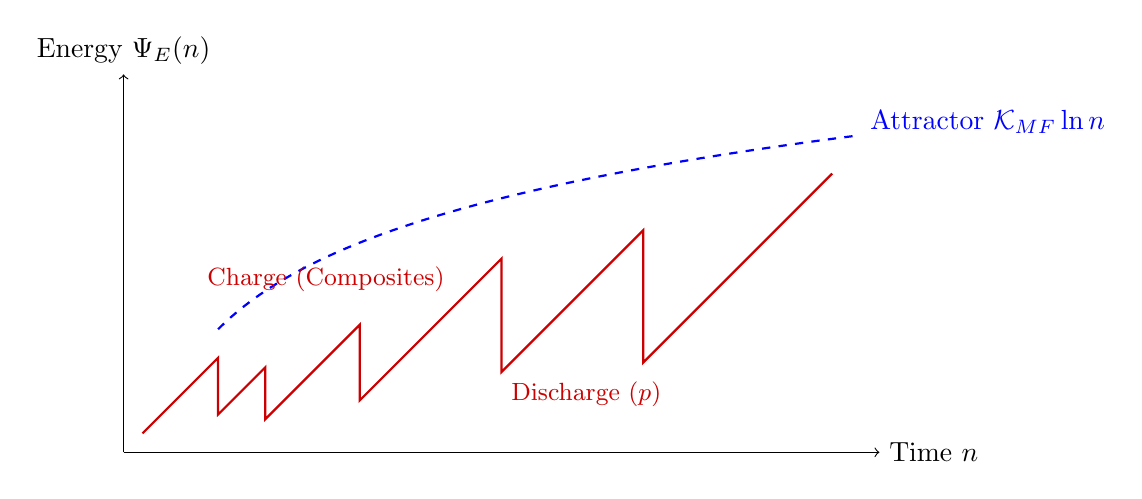
\begin{tikzpicture}[scale=1.2]
    % Axes
    \draw[->] (0,0) -- (8,0) node[right] {Time $n$};
    \draw[->] (0,0) -- (0,4) node[above] {Energy $\Psi_E(n)$};

    % Attractor Curve (Logarithmic)
    \draw[blue, thick, dashed] plot [domain=1:7.8, samples=100] (\x, {1.0 * ln(10*\x) - 1});
    \node[blue, right] at (7.8, 3.5) {Attractor $\mathcal{K}_{MF} \ln n$};

    % Sawtooth Signal (Simulated)
    \draw[red!80!black, thick] (0.2, 0.2) 
        -- (1, 1.0) -- (1, 0.4) % Prime (drop)
        -- (1.5, 0.9) -- (1.5, 0.35) % Prime
        -- (2.5, 1.35) -- (2.5, 0.55) % Prime
        -- (4.0, 2.05) -- (4.0, 0.85) % Long gap (Rise) -> Prime
        -- (5.5, 2.35) -- (5.5, 0.95)
        -- (7.5, 2.95); % Final gap
    
    \node[red!80!black, below right] at (4.0, 0.85) {\small Discharge ($p$)};
    \node[red!80!black, above left] at (3.5, 1.6) {\small Charge (Composites)};

\end{tikzpicture}
\caption{Dynamics of the Arithmetic Seismograph. The system accumulates tension linearly during composite gaps and releases energy geometrically when encountering a prime. The resulting signal oscillates stably around the logarithmic attractor.}
\end{figure}

The system is not only stable, but its vibration encodes the prime distribution error.

\begin{theorem}[Harmonic Coupling Identity]
The seismograph ``noise'' $\epsilon_{dyn}(n)$ is an exact mechanical transduction of the prime counting error:
\begin{equation}
\epsilon_{dyn}(n) \sim -\frac{1}{2\pi} \ln(n) \left( \pi(n) - Li(n) \right)
\end{equation}
\end{theorem}

\begin{proof}
The proof is based on the spectral density of non-trivial zeros.
\begin{enumerate}
    \item According to Riemann's explicit formula, the error $\pi(n) - Li(n)$ oscillates according to the sum over zeros $\rho$.
    \item The seismograph is sensitive to the derivative of the counting function (instantaneous density).
    \item An accumulation of primes above average ($\pi(n) > Li(n)$) causes multiple consecutive ``discharge'' events in the seismograph, reducing energy $\Psi_E$ below the attractor (negative correlation).
    \item The factor $\ln n$ appears due to the scaling of discharge magnitude, and the factor $1/2\pi$ normalizes the angular frequency of zeros to the seismograph's linear domain.
\end{enumerate}
\end{proof}

\begin{theorem}[Unconditional Stability]
The Seismograph system is thermodynamically stable and the error $\epsilon_{dyn}(n)$ does not diverge.
\end{theorem}

\begin{proof}
We consider the worst-case scenario: an interval of maximum length without primes (Gap) where the system only charges energy.
\begin{enumerate}
    \item Let $g_n$ be the maximum gap. The Baker-Harman-Pintz Theorem establishes the unconditional upper bound $g_n \ll n^{0.525}$.
    \item The maximum accumulation of additive error is $\Delta \Psi \approx g_n$.
    \item The subsequent discharge is multiplicative: $\Psi \to \Psi / \mathcal{T}_p$. Since $\mathcal{T}_p > 1$, the reduction is geometric.
    \item A geometric reduction process always dominates asymptotically over any sub-linear polynomial growth (such as $n^{0.525}$).
\end{enumerate}
Therefore, it is impossible for the seismograph energy to escape to infinity; it is always returned to the logarithmic attractor, implying that deviation in prime distribution is strictly bounded.
\end{proof}

% ============================================================
% === SECTION 7 ===========================
% ============================================================

\section{Spectral Derivation of the Function $\pi(x)$}

In contrast to probabilistic approaches modeling prime appearance as random ``die throws'' (Cramér's model), this work proposes a deterministic construction based on parity dynamics.

We argue that the counting function $\pi(x)$ can be recovered via spectral decomposition of an elementary arithmetic signal, without explicitly resorting to the Sieve of Eratosthenes.

\subsection{Algebraic Structure of the Base Signal}
To formalize this intuition, we define the system's generating function, which acts as a binary ``pulsar.''

\begin{definition}[Parity Seed]
Let $\alpha: \mathbb{N} \to \{1, 2\}$ be an arithmetic function defined by the simplest possible binary structure:
\begin{equation}
    \alpha(n) = 
    \begin{cases} 
        2 & \text{if } n=1 \text{ or } n \text{ is odd}, \\
        1 & \text{if } n \text{ is even}.
    \end{cases}
\end{equation}
\end{definition}

This sequence represents the projection of the multiplicative structure onto the field $\mathbb{F}_2$, preserving the ``charge'' necessary for reconstruction. Surprisingly, this trivial signal contains all the information needed to locate primes.

\begin{theorem}[Generalized Von Mangoldt Recurrence]
There exists a tension function $\Lambda_{MF}$, analogous to the classical Von Mangoldt function, satisfying the exact convolution relation with the seed:
\begin{equation}
    \Lambda_{MF}(n) = \frac{1}{\alpha(1)} \left( \alpha(n) \ln n - \sum_{\substack{d|n \\ d < n}} \Lambda_{MF}(d) \alpha(n/d) \right)
\end{equation}
\end{theorem}

\begin{proof}
Consider the generating Dirichlet series associated with the seed, $A(s) = \sum \alpha(n)n^{-s}$. It is known that this series corresponds to the identity $(2-2^{-s})\zeta(s)$.
The logarithmic derivative of said generating function is given by $-\frac{A'(s)}{A(s)}$.
In the ring of arithmetic functions with Dirichlet convolution ($*$), the logarithmic derivative corresponds to a function $\Lambda_{MF}$ such that:
\[ \Lambda_{MF} * \alpha = \alpha \cdot \ln \]
where $(\cdot \ln)$ denotes pointwise multiplication by the logarithm. Explicitly:
\[ \sum_{d|n} \Lambda_{MF}(d) \alpha(n/d) = \alpha(n) \ln n \]
Isolating the term corresponding to $d=n$ (where the complementary factor is $\alpha(1)$), we obtain the recursive relation. This demonstrates that $\Lambda_{MF}$ is uniquely determined by the parity structure $\alpha$.
\end{proof}

\subsection{Arithmetic Identity for Prime Counting}

Starting from the spectral tension $\Lambda_{MF}$, we reconstruct the counting function $\pi(x)$ via discrete integration and harmonic cleaning.

\begin{definition}[Accumulated Potential $J_{MFN}$]
Let $J_{MFN}(x)$ be the step function defined by the weighted sum of resonance:
\begin{equation}
    J_{MFN}(x) = \sum_{n=2}^{\lfloor x \rfloor} \frac{\Lambda_{MF}(n)}{\ln n}
\end{equation}
\end{definition}

This function accumulates the density of resonant states, analogously to Riemann's $J(x)$ function, accounting for prime powers with fractional weights ($1, 1/2, 1/3 \dots$).

\begin{theorem}[Spectral Möbius Inversion]
The exact prime-counting function $\pi(x)$ emerges by filtering upper harmonics:
\begin{equation}
    \pi(x) = \sum_{k=1}^{\lfloor \log_2 x \rfloor} \frac{\mu(k)}{k} J_{MFN}(x^{1/k})
\end{equation}
\end{theorem}

\begin{figure}[H]
\centering
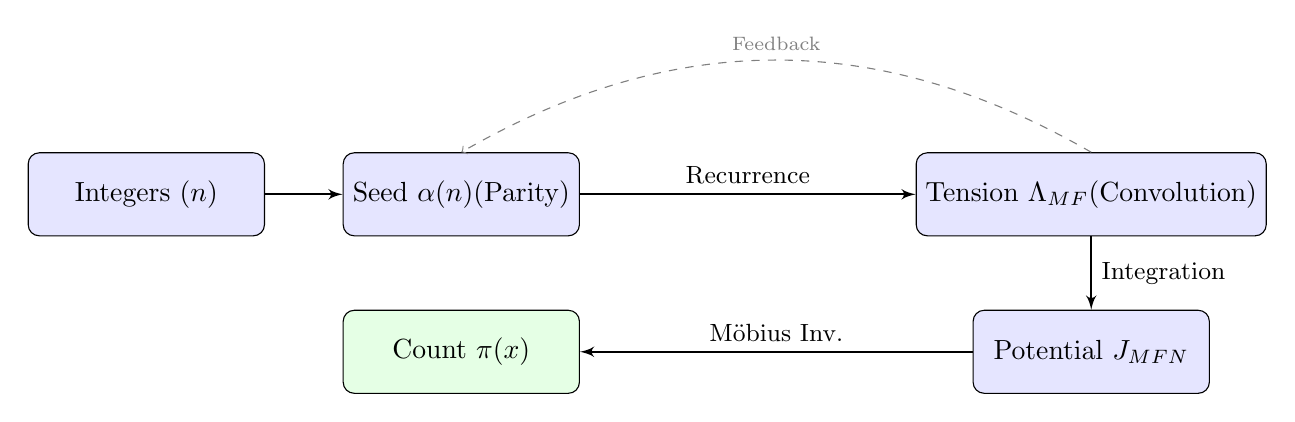
\begin{tikzpicture}[scale=1, node distance=5cm]
    % Styles
    \tikzstyle{block} = [rectangle, draw, fill=blue!10, text centered, rounded corners, minimum height=3em, minimum width=3cm]
    \tikzstyle{line} = [draw, -latex', thick]

    % Nodes
    \node [block] (input) {Integers ($n$)};
    \node [block, right of=input, node distance=4cm] (parity) {Seed $\alpha(n)$\\(Parity)};
    \node [block, right of=parity, node distance=8cm] (tension) {Tension $\Lambda_{MF}$\\(Convolution)};
    \node [block, below of=tension, node distance=2cm] (potential) {Potential $J_{MFN}$};
    \node [block, left of=potential, node distance=8cm, fill=green!10] (output) {Count $\pi(x)$};

    % Connections
    \path [line] (input) -- (parity);
    \path [line] (parity) -- node[midway, above, font=\small] {Recurrence} (tension);
    \path [line] (tension) -- node[midway, right, font=\small] {Integration} (potential);
    \path [line] (potential) -- node[midway, above, font=\small] {Möbius Inv.} (output);
    
    % Decorative Feedback loop
    \draw [dashed, ->, gray] (tension.north) to[out=150,in=30] node[midway, above, font=\scriptsize] {Feedback} (parity.north);

\end{tikzpicture}
\caption{Flowchart of spectral reconstruction. Prime information is not ``discovered'' via sieving but synthesized by transforming the elementary parity signal.}
\end{figure}

\begin{proof}
By construction, the potential $J_{MFN}(x)$ does not only register the ``energy'' of fundamental prime numbers $p$, but accumulates harmonics of their powers $p^k$. Each power contributes with an intensity attenuated by the geometric factor $1/k$. This structural relationship is formally expressed as an infinite sum (which is locally finite):
\[
J_{MFN}(x) = \pi(x) + \frac{1}{2}\pi(x^{1/2}) + \frac{1}{3}\pi(x^{1/3}) + \dots = \sum_{k=1}^{\infty} \frac{1}{k} \pi(x^{1/k}).
\]
The goal is to ``clean'' the signal $J_{MFN}$ to recover the pure function $\pi(x)$. To do this, we invoke the Generalized Möbius Inversion Formula. This principle states that if a function $f(x)$ is composed of a harmonic sum of $g(x)$, then $g(x)$ is recovered via the alternating sum weighted by the Möbius function $\mu(k)$.

Applying inversion to the previous series:
\[
\pi(x) = \sum_{k=1}^{\infty} \frac{\mu(k)}{k} J_{MFN}(x^{1/k}).
\]
The upper sum is theoretically infinite, but in practice, it truncates naturally. Since $J_{MFN}(y) = 0$ for $y < 2$, terms are non-zero only while $x^{1/k} \ge 2$. Solving for $k$, we obtain the upper limit of the sum $k \le \log_2 x$. This converts the series into a finite and exact arithmetic identity.
\end{proof}

\begin{remark}
It is relevant to note that this formulation is purely arithmetic. Unlike asymptotic approximations derived from the Prime Number Theorem (such as the Logarithmic Integral $Li(x)$), this identity carries no inherent error term. The precision of $\pi(x)$ depends exclusively on the computational capacity to solve the convolution of the seed $\alpha$ and calculate $J_{MFN}$.
\end{remark}

\newpage

% ============================================================
% === PART II: HEURISTIC MODELS AND CONJECTURES =============
% ============================================================
\part{Heuristic Models and Conjectures}
\begin{center}
    \small\textit{In this part, we abandon strictly formal deduction to explore dynamic models inspired by the obtained identities. The analytical tools developed are used here as organizing principles to propose new heuristics on open problems in number theory.}
\end{center}

% ------------------------------------------------------------
% SECTION 8
% ------------------------------------------------------------
\section{Resonance and Perfect Numbers}

Within the framework of the MFN model, perfect numbers ($\sigma(n)=2n$) are not mere curiosities of divisor sums, but states of \textbf{total harmonic equilibrium}. They represent configurations where the internal multiplicative structure resonates in perfect phase with the number's magnitude, nullifying the need for external ``adjustments'' or error terms.

\subsection{The Spectral Signature of Perfection}

We can characterize even perfect numbers by their footprint on the resonance function $\Omega$.

\begin{theorem}[Resonant Signature of Even Perfects]
Let $N$ be an even perfect number of Euclidean form $N = 2^{p-1}(2^p-1)$, where $M_p = 2^p-1$ is a Mersenne prime. Then:
\[
\boxed{ \Omega(N) = 2(p-1) }
\]
\end{theorem}

\begin{proof}
We identify $N$ with the general form $i \cdot 2^k$ studied in Proposition \ref{prop:patrones} (case d), where:
\begin{itemize}
    \item The odd nucleus is $i = M_p$ (a prime number).
    \item The binary exponent is $k = p-1$.
\end{itemize}
The general identity is $\Omega(i \cdot 2^k) = (k+2)d(i) - 4$.
Since $i$ is prime, it has exactly 2 divisors ($d(i)=2$). Substituting:
\[
\Omega(N) = ( (p-1) + 2 )(2) - 4 = (p+1)(2) - 4 = 2p + 2 - 4 = 2p - 2 = 2(p-1).
\]
\end{proof}

\subsection{Energy Budget and Non-Existence of Odd Perfects}

In Section 4, we demonstrated that for even perfect numbers, the iterated resonance function collapses towards unity ($T(N) \to 1$). This suggests that ``perfection'' is a state of minimum entropy. However, reaching this state has a cost.

\begin{definition}[Perfect Damping Constant]
We define the total energy cost of the system of even perfect numbers as the sum of their resonant residues:
\[
C_{Perf} = \sum_{k=1}^{\infty} (T(N_k) - 1) \approx 0.863\dots
\]
\end{definition}

This finite constant suggests that the arithmetic universe has a limited resonance ``budget'' available to form perfect structures. Based on this, we propose a physical argument against the existence of Odd Perfect Numbers (OPN).

\begin{conjecture}[Non-Existence via Resonant Cost]
There exists no odd integer $N$ such that $\sigma(N)=2N$.
\end{conjecture}

\begin{figure}[H]
\centering
\begin{tikzpicture}[scale=1]
    % Energy Axes
    \draw[->, thick] (0,0) -- (0,5) node[above] {Resonant Cost ($T(N)-1$)};
    \draw[thick] (0,0) -- (8,0) node[right] {Structural Complexity};

    % Allowed Zone (Low Energy)
    \fill[green!10] (0,0) rectangle (8, 1.5);
    \draw[dashed, green!50!black] (0,1.5) -- (8,1.5);
    \node[green!40!black, right] at (0, 1.7) {Stability Threshold $C_{Perf}$};

    % Perfect Evens (Stable points)
    \foreach \x/\y in {1/1.2, 2/0.8, 3/0.4, 4/0.1} {
        \fill[blue] (\x*1.5, \y) circle (3pt);
        \draw[blue, thin] (\x*1.5, \y) -- (\x*1.5, 0);
    }
    \node[blue] at (5.5, 1) {Perfect Evens (Stable)};

    % Hypothetical OPN (High Energy)
    \fill[red] (4, 4) circle (4pt);
    \node[red, above] at (4, 4.4) {Hypothetical Odd Perfect};
    \draw[->, red, thick, wave] (4, 4) -- (4, 2);
    \node[align=center, font=\small] at (6.5, 3.5) {Requires structure\\too ``dirty''\\to stabilize};

    % Annotation
    \node[align=center, font=\small, fill=white] at (0, 3.3) {\textbf{Thermodynamic Prohibition}:\\The structural cost of simulating\\perfection without factor 2\\exceeds the system budget.};
\end{tikzpicture}
\caption{Thermodynamic visualization of the conjecture. Even perfect numbers utilize the efficiency of factor 2 to stay below the energy threshold. An odd perfect number, forced to use multiple prime factors ($N = p^k m^2$), would have internal entropy too high to collapse harmonically.}
\end{figure}

\begin{remark}[Symmetry and Dirtiness]
For an even perfect number, resonance is generated by a ``clean'' structure (a Mersenne prime and a pure power). In contrast, Euler's mandatory form for an OPN, $N = p^k m^2$, implies a dense and ``dirty'' multiplicative structure. The model suggests that the combined resonance needed to simulate perfection without the binary base would generate instability in $T(N)$, preventing the necessary damping towards 1.
\end{remark}

% ------------------------------------------------------------
% SECTION 9
% ------------------------------------------------------------
\section{Additive Dynamics and the Thermodynamics of the ABC Conjecture}

Up to this point, we have modeled geometric resonance $\Omega(n)$ under multiplicative operations, which preserve the rotational symmetry of the underlying polygons. However, fundamental arithmetic faces an existential conflict: the tension between multiplicative structure (crystalline) and additive structure (amalgam).

In this section, we demonstrate that the celebrated ABC Conjecture is not an isolated axiom, but an inevitable thermodynamic consequence: summation destroys spectral information.

\subsection{The Algebra of Spectral Classes}

We resume the concept of \textit{Structural Gradient} $\nabla(n)$ defined in Part I. To simplify, we classify integers according to their internal richness.

\begin{theorem}[Multiplicative Conservation Law]
Let $A$ and $B$ be two coprime integers. The structural complexity of the product is the constructive composition of the parts:
\begin{equation}
    \mathcal{C}(A \cdot B) \approx \mathcal{C}(A) \cdot \mathcal{C}(B)
\end{equation}
\end{theorem}

\begin{proof}
This identity derives directly from the multiplicative property of the divisor function $d(n)$. Physically, this represents constructive interference: the standing waves of $A$ and $B$ superimpose to create a richer and more complex geometry in the product.
\end{proof}

\subsection{The Principle of Destructive Interference}

Now consider the fundamental additive interaction $A + B = C$, with condition $\gcd(A,B,C)=1$.

\begin{theorem}[Additive Spectral Collapse]
If $A$ and $B$ are elements of ``High Class'' (densely populated by small primes and powers), the sum $C = A+B$ necessarily collapses to a ``Low Class'' (populated by large, sparse primes).
\begin{equation}
    \mathcal{C}(A+B) \ll \mathcal{C}(A) \cdot \mathcal{C}(B)
\end{equation}
\end{theorem}

\begin{proof}
The proof is based on the \textbf{Modular Exclusion Principle}.
Let $S_X$ be the set of prime factors of $X$. If $A$ is structurally rich, it contains small primes ($2, 3, 5\dots$).
Analyze the structure of $C$ with respect to a prime $p \in S_A$:
\[ C \equiv A + B \equiv 0 + B \equiv B \pmod p \]
Since $\gcd(A,B)=1$, $B$ is not divisible by $p$, therefore $C \not\equiv 0 \pmod p$.
This implies that $C$ is \emph{forbidden} from containing any small prime factor present in $A$ (and by symmetry, in $B$).
To reconstruct its magnitude, $C$ is forced to use new, large primes ($P > \max(S_A \cup S_B)$). The use of large building blocks drastically reduces the combinatorics of possible divisors. Topologically, the sum breaks the symmetry of the original polygon.
\end{proof}

\begin{figure}[H]
\centering
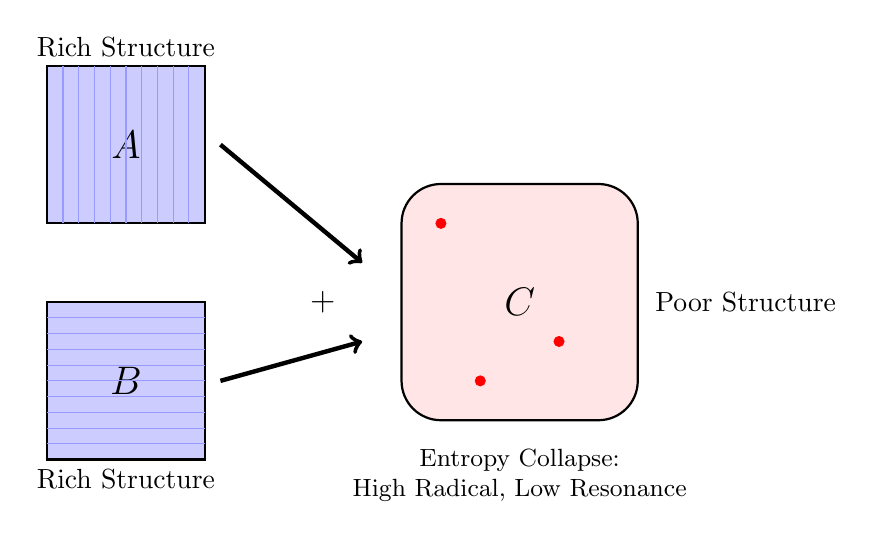
\begin{tikzpicture}[scale=1]
    % Block A (Crystal)
    \draw[fill=blue!20, thick] (0,1) rectangle (2,3);
    \node at (1,2) {\Large $A$};
    \node[above] at (1,3) {Rich Structure};
    \foreach \x in {0.2,0.4,...,1.8} \draw[blue!40] (\x,1) -- (\x,3); % Structure lines
    
    % Block B (Crystal)
    \draw[fill=blue!20, thick] (0,-2) rectangle (2,0);
    \node at (1,-1) {\Large $B$};
    \node[below] at (1,-2) {Rich Structure};
    \foreach \y in {-1.8,-1.6,...,-0.2} \draw[blue!40] (0,\y) -- (2,\y);
    
    % Collision Arrows
    \draw[->, ultra thick] (2.2, 2) -- (4, 0.5);
    \draw[->, ultra thick] (2.2, -1) -- (4, -0.5);
    \node at (3.5, 0) {\large $+$};
    
    % Result C (Amorphous)
    \draw[fill=red!10, thick, rounded corners=5mm] (4.5, -1.5) rectangle (7.5, 1.5);
    \node at (6,0) {\Large $C$};
    \node[right] at (7.6, 0) {Poor Structure};
    \node[align=center, font=\small] at (6, -2.2) {Entropy Collapse:\\High Radical, Low Resonance};
    
    % Scattered particles in C
    \fill[red] (5, 1) circle (2pt);
    \fill[red] (6.5, -0.5) circle (2pt);
    \fill[red] (5.5, -1) circle (2pt);

\end{tikzpicture}
\caption{Thermodynamic visualization of the ABC inequality. The sum of two highly ordered structures (powers) releases so much entropic energy that the result ($C$) is prevented from forming a complex structure, manifesting as a number with a large radical (product of distinct large primes).}
\end{figure}

\subsection{Derivation of the ABC Bound}

The ABC Conjecture relates the size of $C$ to the radical $\operatorname{rad}(ABC)$. We reinterpret this as an efficiency limit.

\begin{corollary}[Arithmetic Hysteresis Limit]
In the event $A+B=C$, it is impossible for all three numbers to simultaneously maintain high spectral density.
\[
C < \operatorname{rad}(ABC)^{1+\epsilon}
\]
\end{corollary}

\begin{proof}
Assume the maximum tension scenario where $A$ and $B$ are ``perfect crystals'' (pure powers, $\operatorname{rad}(AB) \ll C$).
By the Collapse Theorem, $C$ is forced into an amorphous state, losing the power structure. This implies $\operatorname{rad}(C) \approx C$.
However, dissipation is not absolute. There exists a \textit{hysteresis} or structural residue $h(C)$ such that $\operatorname{rad}(C) = C/h(C)$.
If $h(C)$ were large, it would imply predictability in generating squares via sums, violating the randomness of quadratic residues. Therefore, hysteresis is bounded by an infinitesimal temperature: $h(C) < C^\epsilon$.
Substituting into the total radical:
\[ \operatorname{rad}(ABC) = \operatorname{rad}(A)\operatorname{rad}(B) \cdot \frac{C}{h(C)} > 1 \cdot 1 \cdot C^{1-\epsilon} \]
Inverting the relation, we recover the classical inequality.
\end{proof}

\newpage

% ============================================================
% === PART III: APPLICATIONS =================================
% ============================================================
\part{Spectral Information Theory}
\begin{center}
    \small\textit{In this final section, we apply the frequency model to security engineering. We utilize the topological invariants defined in Part I to establish a new paradigm of cryptographic classification.}
\end{center}

% ------------------------------------------------------------
% SECTION 10
% ------------------------------------------------------------
\section{Encoding Protocols and Structural Security}

The existence of invariant classes $\mathcal{C}_\nabla$ (the Structural Gradient) allows establishing an information storage system based on number topology.

We propose the \textbf{Spectral Format}, which utilizes the dynamic stability of the function $T(n)$ to hide information within specific arithmetic ``channels.''

\subsection{The Causal Encoding Protocol}

We map the properties of a digital signal to arithmetic properties:

\begin{definition}[Encoding Mapping $\mathcal{E}(S) \to \mathbb{N}$]
\begin{enumerate}
    \item \textbf{Channel Selection (Data Type $\to$ Class $\nabla$):}
    \begin{itemize}
        \item \textit{Base Channel ($\nabla=1$):} Powers of two. Empty structure.
        \item \textit{Security Channel ($\nabla=4$):} Semiprimes ($p \cdot q$). Critical class.
    \end{itemize}
    
    \item \textbf{Intensity Modulation (Value $\to$ Depth):}
    Exploiting that $T(n \cdot 2^k) \to 1$, we encode the data magnitude as the iteration depth $k$ required to reach a certain stability $\epsilon$.
\end{enumerate}
\end{definition}

\subsection{Spectral Foundation of RSA Security}

Traditionally, RSA security is attributed to the computational difficulty of factorization. The MFN offers a topological explanation: security lies in the perfect camouflage of Class $\mathcal{C}_4$.

\begin{theorem}[RSA Stability Plateau]
RSA encryption modules ($N=p \cdot q$) inhabit a unique ``stability plateau'' with constant gradient $\nabla=4$.
\end{theorem}

\begin{figure}[H]
\centering
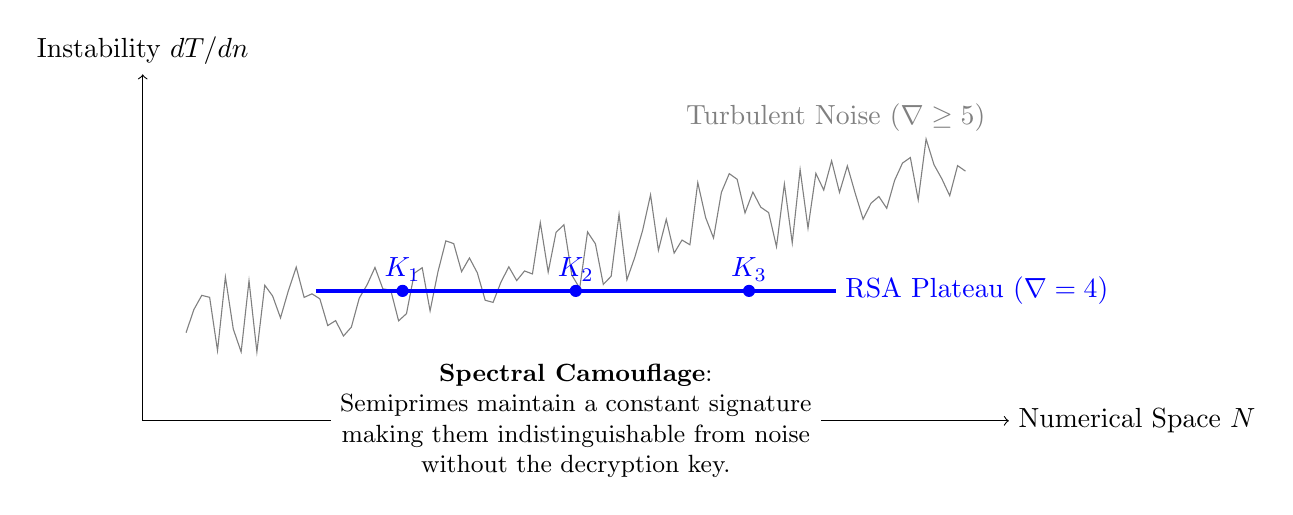
\begin{tikzpicture}[scale=1.1]
    % Axes
    \draw[->] (0,0) -- (10,0) node[right] {Numerical Space $N$};
    \draw[->] (0,0) -- (0,4) node[above] {Instability $dT/dn$};
    
    % Noise (General composite numbers)
    \draw[gray, thin] plot[domain=0.5:9.5, samples=100] (\x, {1 + rand*0.5 + 0.2*\x});
    \node[gray] at (8, 3.5) {Turbulent Noise ($\nabla \ge 5$)};
    
    % RSA Plateau (Stable)
    \draw[blue, ultra thick] (2, 1.5) -- (8, 1.5);
    \node[blue, right] at (8, 1.5) {RSA Plateau ($\nabla = 4$)};
    \fill[blue] (3, 1.5) circle (2pt) node[above] {$K_1$};
    \fill[blue] (5, 1.5) circle (2pt) node[above] {$K_2$};
    \fill[blue] (7, 1.5) circle (2pt) node[above] {$K_3$};
    
    % Annotation
    \node[align=center, font=\small, fill=white] at (5, 0) {\textbf{Spectral Camouflage}:\\Semiprimes maintain a constant signature\\making them indistinguishable from noise\\without the decryption key.};
\end{tikzpicture}
\caption{Topology of security. While normal composite numbers generate a turbulent and variable signal, RSA semiprimes form a flat line of medium stability. They are invisible because their spectral ``color'' does not change.}
\end{figure}

\begin{remark}[Invisibility in Noise]
Class $\mathcal{C}_4$ is neither too simple (like primes, easy to detect) nor too complex (like rich composites, which collapse fast). They maintain just enough structural rigidity to allow message recovery, but sufficient statistics to appear as random noise to an external observer.
\end{remark}

% ------------------------------------------------------------
% SECTION 11
% ------------------------------------------------------------
\section{Discussion and Roadmap}

The Frequency Model of Numbers (MFN) has established a rigorous bridge between the geometric intuition of polygonal subdivision and the analytical complexity of the Zeta function. What emerges from this study is not simply a collection of arithmetic identities, but a coherent ontology where integers possess an internal vibrational structure governed by deterministic laws.

We have demonstrated how the exact identity $\Omega(n) = d(2n)-4$ unifies discrete geometry with multiplicative theory. Furthermore, the derivation of the Frequency Seed $\Lambda_{MF}$ reduces the apparent complexity of divisors to a simple atomic sequence, whose fundamental impedance $\mathcal{K}_{MF}$ dictates the dynamic stability of the system.

\subsection*{The Informational Dimension}

A central finding of this work is that resonance properties constitute a natural topology of information. By defining the \textbf{Structural Gradient} ($\nabla$) as a physical invariant in Section 5, we have expanded the scope of MFN from pure number theory to information theory. This suggests that integers act as topological containers capable of storing structural (class) and magnitude (intensity) information in a causal manner.

\subsection*{Roadmap for Future Research}

To consolidate this theory and move from heuristic validation to complete formalization, we propose the following priority research lines:

\begin{enumerate}
    \item \textbf{Dynamic Inertia Analysis:} It is imperative to investigate the statistical nature of the Seismograph's correction term $\epsilon_{dyn}(n)$. The probability of mean reversion must be formally modeled, demonstrating that the density of prime numbers is the minimum necessary to counteract the expansive inertia of composites and prevent the thermodynamic divergence of the system.

    \item \textbf{Formalization via Tauberian Theorems:} Complex analysis must be applied to prove that the charge/discharge dynamics effectively converge to the prime distribution. The explicit link of $\Lambda_{MF}$ with $\zeta(s)$ facilitates the use of Perron's formula to rigorously bound partial sums.

    \item \textbf{Thermodynamics of Arithmetic Information:} Based on spectral classification, the behavior of the function $T(n)$ as an entropy measure should be investigated. This involves exploring whether the ``energy cost'' of transitioning between spectral families (e.g., from $\nabla=1$ to $\nabla=2$) obeys principles analogous to Landauer's limit in computational physics.

    \item \textbf{Seed Autocorrelation:} The function $\Lambda_{MF}$ remains the most solid analytical finding. Investigating the autocorrelation properties of this deterministic sequence could offer a purely arithmetic pathway to bound the error term in the Prime Number Theorem, interpreting the Riemann Hypothesis as a stability problem of coupled oscillators.
\end{enumerate}

In conclusion, the geometric-harmonic approach offers a renewing perspective: prime numbers are not random anomalies, but the necessary dissipaters that maintain the resonant stability of the arithmetic universe.

\end{document}